\subsection{Calibration Penetrations}
\label{sec:FTs}

The current cryostat design for the %DUNE SP FD 
\spmod with penetrations for various sub-systems is shown in Figure~\ref{fig:ftmap}. The penetrations dedicated for calibrations are highlighted in black circles. The ports on far east and far west are located outside the field cage. The current plan is to use these penetrations for multiple purposes. For example, the penetrations on the far east and west will be used both by laser and radioactive source deployment systems. In addition to these dedicated ports, the Detector Support System (DSS) and cryogenic ports (orange and blue dots in Figure~\ref{fig:ftmap}, respectively) will also be used as needed to route cables for the single phase photon detector calibration system. The DSS and cryogenic ports are accommodated with feedthroughs with a CF63 side flange for this purpose.   

\begin{figure}[tbp]
\centering
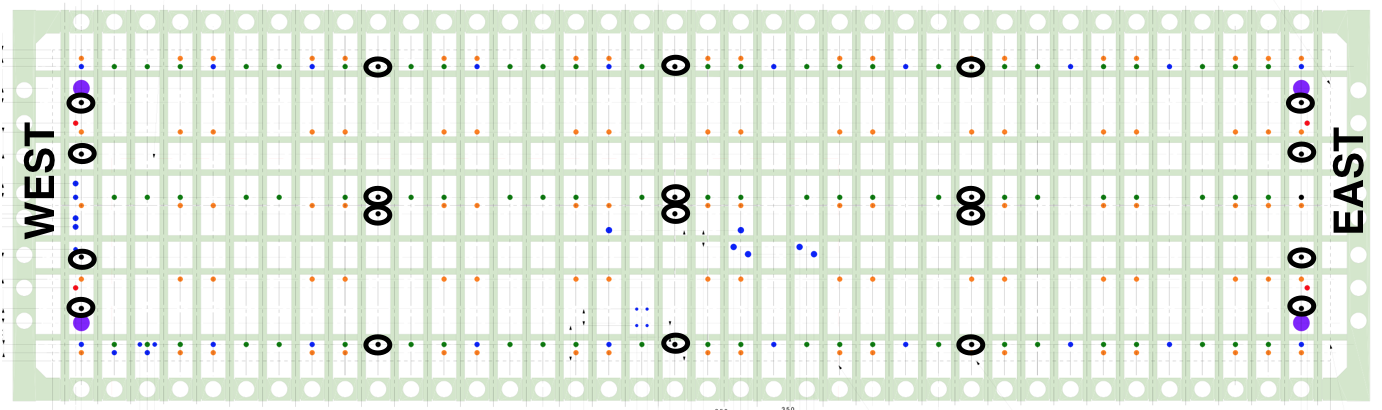
\includegraphics[height=2.0in]{FTmap.png}
\caption{Top view of the \spmod %DUNE SP FD 
cryostat showing various penetrations. Highlighted in black circles are multi-purpose calibration penetrations. The orange dots are TPC signal cable penetrations. The blue ports are \dword{dss} %Detector Support System 
penetrations. The orange ports are TPC signal cable penetrations. The larger purple ports at the four corners of the cryostat are manholes.}
\label{fig:ftmap}
\end{figure}

The placement of these penetrations is largely driven by the ionization track laser and radioactive source system requirements. The ports that are closer to the center of the cryostat 
%\fixme{closer to the center? "inwords of" is not clear to me} resolved
are placed near the APAs (similarly to what is planned for SBND) to minimize any risks due to the HV discharge. For the far east and west ports, HV is not an issue as they are located outside the \dword{fc} and the penetrations are located near mid-drift to meet radioactive source requirements. Implementation of the ionization track laser system proposed in Section~\ref{sec:laser}, requires 20 feedthroughs to cover the four TPC drift volumes; %and 
%this would provide (almost) full volume calibration of the electric field % map 
%and associated diagnostics (e.g., HV). This arrangement gives crossing laser tracks which are necessary to unambiguously construct the field map. 
this arrangement would provide (almost) full volume calibration of the electric field 
and associated diagnostics (e.g. HV). The crossing laser tracks are necessary to unambiguously construct the field map. 

The distance between any two consecutive feedthrough columns in Figure~\ref{fig:ftmap} is assumed to be about \SI{15}{\m}. This is considered %a reasonable assumption 
reasonable since the experience from the \microboone laser system has shown that tracks will propagate over %the 
that detector's full \SI{10}{\m} length. % of the detector. 
Assuming that the effects of Rayleigh scattering and self-focusing (Kerr effect) do not limit the laser track length, %the current 
this laser arrangement could illuminate the full volume with crossing track data. 
It is important to note that at this point in time, a maximum usable track length is unknown and it is not excluded that the full \SI{60}{\m} \detmodule length could be achieved by the laser system after optimization.

The calibration group focused on finalizing the cryostat penetrations for the \spmod driven by the cryostat design timeline. In the near future, a similar exercise will be done to finalize \dpmod %cryostat 
penetrations for calibrations.

%check with KM if she mentioned this and also the SBND system and bring across how this technology can really develop over the SBN era. 
%MicroBooNE has been instrumented with a laser system, but precision results from this system are not yet publicly available as the analysis is ongoing. 
